\documentclass[letterpaper]{article}\usepackage[]{graphicx}\usepackage[]{color}
%% maxwidth is the original width if it is less than linewidth
%% otherwise use linewidth (to make sure the graphics do not exceed the margin)
\makeatletter
\def\maxwidth{ %
  \ifdim\Gin@nat@width>\linewidth
    \linewidth
  \else
    \Gin@nat@width
  \fi
}
\makeatother

\definecolor{fgcolor}{rgb}{0.396, 0.482, 0.514}
\newcommand{\hlnum}[1]{\textcolor[rgb]{0.863,0.196,0.184}{#1}}%
\newcommand{\hlstr}[1]{\textcolor[rgb]{0.863,0.196,0.184}{#1}}%
\newcommand{\hlcom}[1]{\textcolor[rgb]{0.576,0.631,0.631}{#1}}%
\newcommand{\hlopt}[1]{\textcolor[rgb]{0.345,0.431,0.459}{#1}}%
\newcommand{\hlstd}[1]{\textcolor[rgb]{0.396,0.482,0.514}{#1}}%
\newcommand{\hlkwa}[1]{\textcolor[rgb]{0.796,0.294,0.086}{#1}}%
\newcommand{\hlkwb}[1]{\textcolor[rgb]{0.522,0.6,0}{#1}}%
\newcommand{\hlkwc}[1]{\textcolor[rgb]{0.796,0.294,0.086}{#1}}%
\newcommand{\hlkwd}[1]{\textcolor[rgb]{0.345,0.431,0.459}{#1}}%

\usepackage{framed}
\makeatletter
\newenvironment{kframe}{%
 \def\at@end@of@kframe{}%
 \ifinner\ifhmode%
  \def\at@end@of@kframe{\end{minipage}}%
  \begin{minipage}{\columnwidth}%
 \fi\fi%
 \def\FrameCommand##1{\hskip\@totalleftmargin \hskip-\fboxsep
 \colorbox{shadecolor}{##1}\hskip-\fboxsep
     % There is no \\@totalrightmargin, so:
     \hskip-\linewidth \hskip-\@totalleftmargin \hskip\columnwidth}%
 \MakeFramed {\advance\hsize-\width
   \@totalleftmargin\z@ \linewidth\hsize
   \@setminipage}}%
 {\par\unskip\endMakeFramed%
 \at@end@of@kframe}
\makeatother

\definecolor{shadecolor}{rgb}{.97, .97, .97}
\definecolor{messagecolor}{rgb}{0, 0, 0}
\definecolor{warningcolor}{rgb}{1, 0, 1}
\definecolor{errorcolor}{rgb}{1, 0, 0}
\newenvironment{knitrout}{}{} % an empty environment to be redefined in TeX

\usepackage{alltt}
%\VignetteIndexEntry{Migration from poppr version 1}
%\VignetteEngine{knitr::knitr}
\usepackage{graphicx}
\usepackage[colorlinks = true,
            urlcolor = blue,
            citecolor = blue,
            linkcolor = blue]{hyperref}
\usepackage{array}
\usepackage{color}
\usepackage[usenames,dvipsnames,svgnames,table]{xcolor}
\usepackage[utf8]{inputenc} % for UTF-8/single quotes from sQuote()
\usepackage{fullpage}
\usepackage{mathtools}
\usepackage{makeidx}
\usepackage{longtable}

% for bold symbols in mathmode
\usepackage{bm}
\newcommand{\R}{\mathbb{R}}
\newcommand{\m}[1]{\mathbf{#1}}
\newcommand{\tab}{\hspace*{1em}}
\newcolumntype{H}{>{\setbox0=\hbox\bgroup} c<{\egroup}@{}}
\newcommand{\cmdlink}[2]{%
  \texttt{\hyperref[#1]{#2}}%
}
\newcommand{\seclink}[2]{%
  \textsc{\hyperref[#1]{#2}}%
}

\newcommand{\poppr}{\textit{poppr}}
\newcommand{\Poppr}{\textit{Poppr}}
\newcommand{\adegenet}{\textit{adegenet}}
\newcommand{\Adegenet}{\textit{Adegenet}}
\newcommand{\tline}{
  \noindent
  \rule{\textwidth}{1pt}
  \par
}
\newcommand{\bline}{
  \noindent
  \rule{\textwidth}{1pt}
  \kern1pt
}

\newcommand{\jala}{
  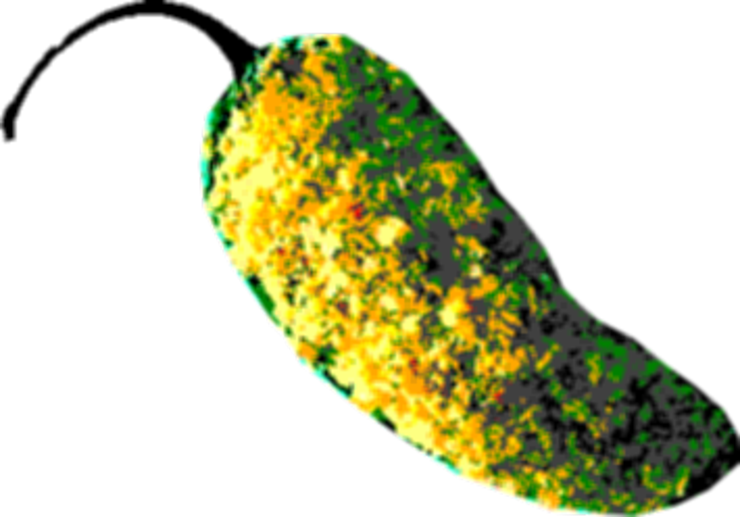
\includegraphics[height = 5mm, keepaspectratio=true]{jalapeno-poppers}
}

\newcommand{\revjala}{
  \scalebox{-1}[1]{\jala{}}
}

\title{Migration from poppr version 1.1 to 1.1.5.99.542}
\author{Zhian N. Kamvar$^{1}$\ and Niklaus J. Gr\"unwald$^{1,2}$\\\scriptsize{1)
Department of Botany and Plant Pathology, Oregon State University, Corvallis,
OR}\\\scriptsize{2) Horticultural Crops Research Laboratory, USDA-ARS,
Corvallis, OR}}
\IfFileExists{upquote.sty}{\usepackage{upquote}}{}
\begin{document}
% Set the width of figures.
\setkeys{Gin}{width=0.5\textwidth}





\definecolor{light-gray}{gray}{0.97}
\definecolor{salmon}{HTML}{F0AAAA}

\maketitle 
\begin{abstract} 
In 2015, \adegenet{} and \poppr{} both went through major, breaking changes.
In this short vignette, we will demonstrate the \texttt{old2new\_} family of
functions that will convert your data and provide a guide of functions that have
changed name or functionality. 
\end{abstract} 
% Inserting the \Poppr{} logo here 

\begin{figure}[b]   
  \centering
  \label{logo}   
  
\includegraphics{popprlogo} 
\end{figure} 

\newpage 
\begingroup
  \hypersetup{linkcolor=black} 
  \tableofcontents 
\endgroup 

%\linenumbers
\section{Introduction}

In March of 2015, a population genetics in R hackathon was held at NESCent in 
Durham, North Carolina, USA. Details can be found here: 
\url{https://github.com/NESCent/r-popgen-hackathon}. This hackthon identified 
several issues concerning population genetics in R, one of them being the need
for package efficiency. Thus, many packages, including \adegenet{} and \poppr{}
received major updates \cite{kamvar2015novel}. The side effect of these updates 
is that backwards compatibility has been broken in making \adegenet{} and 
\poppr{} more efficient.

\subsection{Color Schemes}

Because this vignette will discuss both code that will work and code that will
is not recommended, we will use two color schemes to distinguish the two. Note
that all code that will fail is wrapped in a \texttt{try()} command.
\begin{itemize}
\item \textbf{Solarized-light theme for code that works}:
\begin{knitrout}
\definecolor{shadecolor}{rgb}{0.992, 0.965, 0.89}\color{fgcolor}\begin{kframe}
\begin{alltt}
\hlkwd{rnorm}\hlstd{(}\hlnum{10}\hlstd{)} \hlcom{# Works!}
\end{alltt}
\begin{verbatim}
##  [1] -0.08032641  1.62675973 -1.44217738  1.57439313 -0.63546070
##  [6] -1.93335850  0.90089598  0.24635874 -0.55116211 -0.32472416
\end{verbatim}
\end{kframe}
\end{knitrout}



\item \textbf{Solarized-dark theme for code that is not recommended}:
\begin{knitrout}
\definecolor{shadecolor}{rgb}{0, 0.169, 0.212}\color{fgcolor}\begin{kframe}
\begin{alltt}
\hlkwd{try}\hlstd{(}\hlkwd{rnorm}\hlstd{(}\hlstr{"A"}\hlstd{))} \hlcom{# Throws a warning and error.}
\end{alltt}


{\ttfamily\noindent\color{warningcolor}{\#\# Warning in rnorm("{}A"{}): NAs introduced by coercion}}\end{kframe}
\end{knitrout}


\end{itemize}
\subsection{Major changes in \adegenet{}}

Major breaking changes involve the structure of the \adegenet{}'s \textsc{genind}
object. The \texttt{@tab} slot has been changed from containing allelic frequency
data to counts of alleles, thus reducing the size of the data by half. Several
redundant slots have also disappeared including \texttt{@pop.names}, 
\texttt{@loc.names}, and \texttt{@ind.names}. The function \texttt{na.replace()}
has been removed and modification of the data set directly is discouraged. 

\subsection{Major changes in \poppr{}}

The function \texttt{splitcombine()} has officially been removed (it was 
deprecated in version 1.1). Version 1.1 introduced the \texttt{@hierarchy} slot
to contain population hierarchies. This slot was moved to the \textsc{genind}
object and renamed to \texttt{@strata}. To make things particularly complicated,
a slot called \texttt{@hierarchy} was also added to the \textsc{genind} object,
but it only contains a formula. All methods associated with the previous
hierarchy slot (e.g. \texttt{splithierarchy()} or \texttt{setpop()}) still exist
in \poppr{} as a wrapper to the true methods. 

\section{Migrating data}

Migrating data from 1.1 to 2.0 is simple, all you have to do is use the function
\texttt{old2new\_genind()} or \texttt{old2new\_genclone()} depending on the type
of data you have. Below is an example of using these functions on old data.

\subsection{migrating genind data}

We will use the \texttt{partial\_clone} data set from \poppr{} version 1.1.5
for demonstration. First, we'll load the data.

\begin{knitrout}
\definecolor{shadecolor}{rgb}{0.992, 0.965, 0.89}\color{fgcolor}\begin{kframe}
\begin{alltt}
\hlkwd{library}\hlstd{(}\hlstr{"poppr"}\hlstd{)}
\end{alltt}


{\ttfamily\noindent\itshape\color{messagecolor}{\#\# Loading required package: adegenet\\\#\# Loading required package: ade4\\\#\# \\\#\#\ \ \ \ /// adegenet 2.0.0 is loaded ////////////\\\#\# \\\#\#\ \ \ \ > overview: '?adegenet'\\\#\#\ \ \ \ > tutorials/doc/questions: 'adegenetWeb()' \\\#\#\ \ \ \ > bug reports/feature resquests: adegenetIssues()\\\#\# \\\#\# \\\#\# This is poppr version 1.1.5.99.542. To get started, type package?poppr}}\begin{alltt}
\hlkwd{data}\hlstd{(}\hlstr{"old_partial_clone"}\hlstd{,} \hlkwc{package} \hlstd{=} \hlstr{"poppr"}\hlstd{)} \hlcom{# From version 1.1.5}
\hlkwd{data}\hlstd{(}\hlstr{"partial_clone"}\hlstd{,} \hlkwc{package} \hlstd{=} \hlstr{"poppr"}\hlstd{)}     \hlcom{# From version 2.0.0}
\end{alltt}
\end{kframe}
\end{knitrout}

Now, let's examine the names of the slots and compare it with the current 
version.

\begin{knitrout}
\definecolor{shadecolor}{rgb}{0.992, 0.965, 0.89}\color{fgcolor}\begin{kframe}
\begin{alltt}
\hlkwd{names}\hlstd{(}\hlkwd{attributes}\hlstd{(old_partial_clone))}         \hlcom{# Has pop.names, ind.names, etc.}
\end{alltt}
\begin{verbatim}
##  [1] "tab"       "loc.names" "loc.fac"   "loc.nall"  "all.names"
##  [6] "call"      "ind.names" "pop"       "pop.names" "ploidy"   
## [11] "type"      "other"     "class"
\end{verbatim}
\begin{alltt}
\hlkwd{names}\hlstd{(partial_clone)}                         \hlcom{# Has strata slot.}
\end{alltt}
\begin{verbatim}
##  [1] "tab"       "loc.fac"   "loc.n.all" "all.names" "ploidy"   
##  [6] "type"      "other"     "call"      "pop"       "strata"   
## [11] "hierarchy"
\end{verbatim}
\begin{alltt}
\hlcom{# This is ultimately what we want}
\hlstd{partial_clone}
\end{alltt}
\begin{verbatim}
## /// GENIND OBJECT /////////
## 
##  // 50 individuals; 10 loci; 35 alleles; size: 21.2 Kb
## 
##  // Basic content
##    @tab:  50 x 35 matrix of allele counts
##    @loc.n.all: number of alleles per locus (range: 3-5)
##    @loc.fac: locus factor for the 35 columns of @tab
##    @all.names: list of allele names for each locus
##    @ploidy: ploidy of each individual  (range: 2-2)
##    @type:  codom
##    @call: old2new_genind(object = x, donor = new(class(x)))
## 
##  // Optional content
##    @pop: population of each individual (group size range: 12-13)
\end{verbatim}
\end{kframe}
\end{knitrout}

We can try printing the old object, but it won't work and will throw an error:



\begin{knitrout}
\definecolor{shadecolor}{rgb}{0, 0.169, 0.212}\color{fgcolor}\begin{kframe}
\begin{alltt}
\hlkwd{try}\hlstd{(old_partial_clone)}
\end{alltt}
\begin{verbatim}
## /// GENIND OBJECT /////////
## 
##  // 50 individuals; 10 loci; 35 alleles; size: 35 Kb
## 
##  // Basic content
##    @tab:  50 x 35 matrix of allele counts
\end{verbatim}


{\ttfamily\noindent\bfseries\color{errorcolor}{\#\# Error in .nextMethod(x = x): no slot of name "{}loc.n.all"{} for this object of class "{}genind"{}}}\end{kframe}
\end{knitrout}




To correct this we should use the function \texttt{old2new\_genind()}.

\begin{knitrout}
\definecolor{shadecolor}{rgb}{0.992, 0.965, 0.89}\color{fgcolor}\begin{kframe}
\begin{alltt}
\hlstd{opc} \hlkwb{<-} \hlkwd{old2new_genind}\hlstd{(old_partial_clone)}
\hlstd{opc} \hlcom{# It prints!}
\end{alltt}
\begin{verbatim}
## /// GENIND OBJECT /////////
## 
##  // 50 individuals; 10 loci; 35 alleles; size: 20.7 Kb
## 
##  // Basic content
##    @tab:  50 x 35 matrix of allele counts
##    @loc.n.all: number of alleles per locus (range: 3-5)
##    @loc.fac: locus factor for the 35 columns of @tab
##    @all.names: list of allele names for each locus
##    @ploidy: ploidy of each individual  (range: 2-2)
##    @type:  codom
##    @call: old2new_genind(object = old_partial_clone)
## 
##  // Optional content
##    @pop: population of each individual (group size range: 12-13)
\end{verbatim}
\end{kframe}
\end{knitrout}

Be careful, though. \textbf{Do not use old2new\_genind more than once!}.

\subsection{migrating genclone data}

This procedure is almost exactly the same as migrating genind data. We will use
the \texttt{Pinf} data set for our demonstration.

\begin{knitrout}
\definecolor{shadecolor}{rgb}{0.992, 0.965, 0.89}\color{fgcolor}\begin{kframe}
\begin{alltt}
\hlkwd{data}\hlstd{(}\hlstr{"old_Pinf"}\hlstd{,} \hlkwc{package} \hlstd{=} \hlstr{"poppr"}\hlstd{)} \hlcom{# From version 1.1.5}
\hlkwd{data}\hlstd{(}\hlstr{"Pinf"}\hlstd{,} \hlkwc{package} \hlstd{=} \hlstr{"poppr"}\hlstd{)}     \hlcom{# From version 2.0.0}
\hlkwd{names}\hlstd{(}\hlkwd{attributes}\hlstd{(old_Pinf))}         \hlcom{# No strata slot}
\end{alltt}
\begin{verbatim}
##  [1] "mlg"       "hierarchy" "tab"       "loc.names" "loc.fac"  
##  [6] "loc.nall"  "all.names" "call"      "ind.names" "pop"      
## [11] "pop.names" "ploidy"    "type"      "other"     "class"    
## [16] "strata"
\end{verbatim}
\begin{alltt}
\hlkwd{names}\hlstd{(Pinf)}                         \hlcom{# Has strata slot}
\end{alltt}
\begin{verbatim}
##  [1] "mlg"       "tab"       "loc.fac"   "loc.n.all" "all.names"
##  [6] "ploidy"    "type"      "other"     "call"      "pop"      
## [11] "strata"    "hierarchy"
\end{verbatim}
\begin{alltt}
\hlstd{Pinf}                                \hlcom{# What we want}
\end{alltt}
\begin{verbatim}
## 
## This is a genclone object
## -------------------------
## Genotype information:
## 
##    72 multilocus genotypes
##    86 tetraploid individuals
##    11 codominant loci
## 
## Population information:
## 
##     2 strata - Continent Country
##     2 populations defined - South America North America
\end{verbatim}
\end{kframe}
\end{knitrout}

Again, we can just use \texttt{old2new\_genclone()} to convert this. 

\begin{knitrout}
\definecolor{shadecolor}{rgb}{0.992, 0.965, 0.89}\color{fgcolor}\begin{kframe}
\begin{alltt}
\hlstd{opi} \hlkwb{<-} \hlkwd{old2new_genclone}\hlstd{(old_Pinf)}
\hlstd{opi} \hlcom{# It prints!}
\end{alltt}
\begin{verbatim}
## 
## This is a genclone object
## -------------------------
## Genotype information:
## 
##    72 multilocus genotypes
##    86 tetraploid individuals
##    11 codominant loci
## 
## Population information:
## 
##     2 strata - Continent Country
##     2 populations defined - South America North America
\end{verbatim}
\end{kframe}
\end{knitrout}

\section{Hierarchy functions/accessors}

Since the \texttt{@hierarchy} slot was moved to the \texttt{@strata} slot, the
methods also had to change. Below is a table to guide you from the old to the 
new functions. 

\begin{table}[h]
\centering
\label{stratatable}
\begin{tabular}{lr}
\textbf{old version} & \textbf{new version} \\ \hline
\texttt{sethierarchy()} & \texttt{strata()} \\ 
\texttt{gethierarchy()} & \texttt{strata()} \\ 
\texttt{splithierarchy()} & \texttt{splitStrata()} \\ 
\texttt{addhierarchy()} & \texttt{addStrata()} \\ 
\texttt{namehierarchy()} & \texttt{nameStrata()} \\ 
\texttt{setpop()} & \texttt{setPop()} \\ \hline
\end{tabular}
\caption{Function conversion from version 1.1 to 2.0}
\end{table}

While all of the previous hierarchy functions still exist, they exist in a 
deprecated fashion and will inform you how to properly use them. For example,
if we wanted to use the old function \texttt{gethierarchy()}, it would throw a 
warning:



\begin{knitrout}
\definecolor{shadecolor}{rgb}{0, 0.169, 0.212}\color{fgcolor}\begin{kframe}
\begin{alltt}
\hlkwd{head}\hlstd{(}\hlkwd{gethierarchy}\hlstd{(Pinf,} \hlopt{~}\hlstd{Continent}\hlopt{/}\hlstd{Country))} \hlcom{# Throws warning}
\end{alltt}


{\ttfamily\noindent\color{warningcolor}{\#\# Warning: 'gethierarchy' has been deprecated, moved to the adegenet package, and renamed to 'strata'.\\\#\# \\\#\#\ \ Please use:\\\#\#\ \ strata(Pinf, \textasciitilde{}Continent/Country)}}\begin{verbatim}
##        Continent                Country
## 20 South America South America_Colombia
## 21 South America South America_Colombia
## 22 South America South America_Colombia
## 23 South America South America_Colombia
## 24 South America South America_Colombia
## 25 South America  South America_Ecuador
\end{verbatim}
\end{kframe}
\end{knitrout}


\begin{knitrout}
\definecolor{shadecolor}{rgb}{0.992, 0.965, 0.89}\color{fgcolor}\begin{kframe}
\begin{alltt}
\hlkwd{head}\hlstd{(}\hlkwd{strata}\hlstd{(Pinf,} \hlopt{~}\hlstd{Continent}\hlopt{/}\hlstd{Country))}       \hlcom{# No warning :)}
\end{alltt}
\begin{verbatim}
##        Continent                Country
## 20 South America South America_Colombia
## 21 South America South America_Colombia
## 22 South America South America_Colombia
## 23 South America South America_Colombia
## 24 South America South America_Colombia
## 25 South America  South America_Ecuador
\end{verbatim}
\end{kframe}
\end{knitrout}

Note, the function \texttt{setpop()} is also affected:


\begin{knitrout}
\definecolor{shadecolor}{rgb}{0, 0.169, 0.212}\color{fgcolor}\begin{kframe}
\begin{alltt}
\hlkwd{setpop}\hlstd{(Pinf)} \hlkwb{<-} \hlopt{~}\hlstd{Country} \hlcom{# Ambiguous warning}
\end{alltt}


{\ttfamily\noindent\color{warningcolor}{\#\# Warning: 'setpop' has been deprecated, moved to the adegenet package, and renamed to 'setPop'.\\\#\# \\\#\#\ \ Please use:\\\#\#\ \ setPop()}}\end{kframe}
\end{knitrout}

\begin{knitrout}
\definecolor{shadecolor}{rgb}{0.992, 0.965, 0.89}\color{fgcolor}\begin{kframe}
\begin{alltt}
\hlkwd{setPop}\hlstd{(Pinf)} \hlkwb{<-} \hlopt{~}\hlstd{Country} \hlcom{# No warning}
\end{alltt}
\end{kframe}
\end{knitrout}

For many of the functions where you use the assignment, it can't tell what 
arguments you supply, so it will simply suggest the new function. 


\subsection{Additional warning}

Please read this section if you have code that directly accesses the hierarchy
or strata slot directly. An example is below:

\begin{knitrout}
\definecolor{shadecolor}{rgb}{0, 0.169, 0.212}\color{fgcolor}\begin{kframe}
\begin{alltt}
\hlstd{myData}\hlopt{@}\hlkwc{hierarchy} \hlkwb{<-} \hlstd{myData}\hlopt{@}\hlkwc{hierarchy}\hlstd{[}\hlopt{-}\hlnum{2}\hlstd{]} \hlcom{# wat}
\end{alltt}
\end{kframe}
\end{knitrout}

If you have done such a thing, then migrating to poppr 2.0 will be a bit more 
difficult. The hierarchy slot now has a completely different meaning, as it 
will now simply contain a formula specifying which levels of the strata are
hierarchical. 

My recommendation for this situation is to go through your code and replace all
lines where \texttt{@hierarchy} is used with the proper accessors. This is much
better than other solutions \footnote{For example: a hackish way to fix your
situation is to do a search and replace through your code, replacing all
instances of \texttt{@hierarchy} with \texttt{@strata}}.

\subsubsection{Why should I use the accessors?}

While it may seem reasonable to modify a slot directly, using the accessors is 
ultimately the best way to modify your data because the accessors will always 
verify the incoming data. This is shown in the adegenet basics tutorial (See:
\texttt{adegenetTutorial("basics")}). I will show a short example here with
the Pinf data set, first I will show what happens when you don't use the
accessors:

\begin{knitrout}
\definecolor{shadecolor}{rgb}{0, 0.169, 0.212}\color{fgcolor}\begin{kframe}
\begin{alltt}
\hlstd{newPinf}        \hlkwb{<-} \hlstd{Pinf}
\hlstd{the_strata}     \hlkwb{<-} \hlkwd{head}\hlstd{(newPinf}\hlopt{@}\hlkwc{strata}\hlstd{)}
\hlstd{newPinf}\hlopt{@}\hlkwc{strata} \hlkwb{<-} \hlstd{the_strata}     \hlcom{# Only setting strata for six samples!}
\hlstd{newPinf}\hlopt{@}\hlkwc{strata}                   \hlcom{# How is this allowed?}
\end{alltt}
\begin{verbatim}
##        Continent  Country
## 20 South America Colombia
## 21 South America Colombia
## 22 South America Colombia
## 23 South America Colombia
## 24 South America Colombia
## 25 South America  Ecuador
\end{verbatim}
\begin{alltt}
\hlkwd{try}\hlstd{(}\hlkwd{setPop}\hlstd{(newPinf)} \hlkwb{<-} \hlopt{~}\hlstd{Country)} \hlcom{# Oh.}
\end{alltt}
\end{kframe}
\end{knitrout}
\begin{knitrout}
\definecolor{shadecolor}{rgb}{0, 0.169, 0.212}\color{fgcolor}\begin{kframe}


{\ttfamily\noindent\bfseries\color{errorcolor}{\#\# Error in `pop<-`(`*tmp*`, value = structure(c(1L, 1L, 1L, 1L, 1L, 2L), .Label = c("{}Colombia"{},\ \ : \\\#\#\ \  wrong length for population factor}}\end{kframe}
\end{knitrout}


If we had used accessors, the error would have been caught from the start!

\begin{knitrout}
\definecolor{shadecolor}{rgb}{0.992, 0.965, 0.89}\color{fgcolor}\begin{kframe}
\begin{alltt}
\hlstd{the_strata}       \hlkwb{<-} \hlkwd{head}\hlstd{(}\hlkwd{strata}\hlstd{(Pinf))}
\hlkwd{try}\hlstd{(}\hlkwd{strata}\hlstd{(Pinf)} \hlkwb{<-} \hlstd{the_strata)}
\end{alltt}
\end{kframe}
\end{knitrout}
\begin{knitrout}
\definecolor{shadecolor}{rgb}{0.992, 0.965, 0.89}\color{fgcolor}\begin{kframe}


{\ttfamily\noindent\bfseries\color{errorcolor}{\#\# Error : Number of rows in data frame not equal to number of individuals in object.}}\end{kframe}
\end{knitrout}



\bibliographystyle{plain}
\bibliography{the_bibliography}
\end{document}
